\documentclass{report}

\input{preamble}
\input{macros}
\input{letterfonts}

\title{\Huge{Math 120}}
\author{\huge{PSet 2}}
\date{Sep 12 2024}

\begin{document}

\maketitle
\newpage% or \cleardoublepage
% \pdfbookmark[<level>]{<title>}{<dest>}
\pdfbookmark[section]{\contentsname}{toc}
\tableofcontents
\pagebreak

\chapter{}
\section{PSet 2}

\qs{}{
	\insertpng[0.38]{Prob1.png}
	Find the curve parameterized by each vector-valued function. Justify your answers 
	\begin{enumerate}
		\item[(a)] $\vec{r}(t) = \langle \cos t, \sin t, t \rangle$
		\item[(b)] $\vec{r}(t) = t \langle \cos t, \sin t, t \rangle$
		\item[(c)] $\vec{r}(t) = \langle \cos t, \sin t, t^3 \rangle$
		\item[(d)] $\vec{r}(t) = \langle \cos(t^3), \sin(t^3), t^3 \rangle$
		\item[(e)] $\vec{r}(u) = \langle \cos u, \sin u, 1 + \sin(4u) \rangle$
		\item[(f)] $\vec{r}(u) = \langle \cos u, \sin u, 1 + 4\sin(u) \rangle$
		\item[(g)] $\vec{r}(t) = \langle 2\cos t, 1 + 4 \cos t, 3\cos t \rangle$
	\end{enumerate}
}

\sol{
	\\ Equation a should make a helix with fixed radi lengths so it goes wiht curve I. 
	\\ Equation b is similar to equation a but would have increasing ring sizes as t increases so it goes with curve II. 
	\\ Equation c shou
	\\ Equation d is similar to equation a except the helix would get rings faster. It would still go with curve I. 
	\\ Equation e would go with curve IV because the x and y portions should form circles but due to $1 + \sin(4u)$ there should also be 
	oscillation in the z axis. 
	\\ Equation f would go with curve V because it has oscillating height with periods that match the y-axis. 
	\\ Equation g would go with curve VI because all components are proportional to $\cos t$ which suggests a straight line. 
}



\qs{}{
	Find a vector function that represents the curve of intersection of the plane $z = -2$ and the sphere $x^2 + (y-1)^2 + (z+1)^2 = 9$.
}
\sol{
	\[ x^{2} + (y-1)^{2} + ((-2) + 1)^{2} = 9 \] 
	\[ x^{2} + (y-1)^{2} = 8 \]
	\[ r = 2 \sqrt{2} \]
	\[ x(t) = 2\sqrt{2} \cos (t) \]
	\[ y - 1 = 2\sqrt{2} \sin(t) \Rightarrow y = 2\sqrt{t} \sin(t) + 1 \]
	\[ \vec{r}(t) = \langle 2\sqrt{2} \cos(t), 2\sqrt{2} \sin(t) + 1, -2 \rangle \] 
}
\qs{}{
	Consider the vector-valued function $\vec{r}_1(t) = \langle 2\sin t, -3\cos t, 0 \rangle$, $0 \leq t \leq 2\pi$.
	\begin{enumerate}
		\item[(a)] Sketch the plane curve given by $\vec{r}_1(t)$.
		\item[(b)] Compute and draw on your sketch from part (a) the position vector $\vec{r}_1 \left( \frac{2\pi}{3} \right)$ and the tangent vector $\vec{r}_1' \left( \frac{2\pi}{3} \right)$.
		\item[(c)] The vector-valued function $\vec{r}_2(t) = \langle 2\cos(3t), -3\sin(3t) \rangle$ parameterizes the same curve. Find the smallest $t^* > 0$ such that $\vec{r}_2(t^*) = \vec{r}_1 \left( \frac{2\pi}{3} \right)$, and compute $\vec{r}_2'(t^*)$. Explain how and why $\vec{r}_2'(t^*)$ differs from the tangent vector $\vec{r}_1' \left( \frac{2\pi}{3} \right)$ you computed in part (b). 
	\end{enumerate}
}

\sol{ 
	\\
	b) 
	\[ \vec{r}_{1}'(t) = \langle 2 \cos(t), 3 \sin(t) \rangle  \]
	\[ \vec{r}_{1}\left(\frac{2\pi}{3}\right) = \langle 2 \cos \left(\frac{2 \pi}{3}\right), 3 \sin\left(\frac{2 \pi}{3} \right)\rangle \]  
	\[ \vec{r}_{1}\left(\frac{2\pi}{3}\right) = \langle 2 \left( -\frac{1}{2}\right), 3 \left( \frac{\sqrt{3}}{2} \right)\rangle \] 
	\[  \vec{r}_{1}\left(\frac{2\pi}{3}\right) = \langle -1, \frac{3 \sqrt{3}}{2} \rangle \] 
}

\qs{}{
	Find parametric equations for the tangent line to the curve parameterized by 
	\[
	x = 2t + 1, \quad y = e^{t^2 - 4}, \quad z = \ln(1 + t^2)
	\]
	at the point $(5, 1, \ln 5)$.
}

\sol{
	\[ x(t) = 2(t) + 1 \quad y(t) = e^{t^{2} - 4} \quad z(t) = \ln(1 + t)^{2} \] 
	\[ x'(t) = 2 \quad y'(t) = 2te^{t^{2} - 4} \quad z'(t) = \frac{2t}{1+t^{2}} \]
	\[ 5 = 2t + 1 \Rightarrow 4 = 2t \Rightarrow t = 2\]  
	\[ x'(2) = 2 \quad y'(2) =  4e^{2^{2}-4} = 4 \quad z'(t) = \frac{4}{5} \] 
	\[ x: 5 + 2t \quad y: 1 + 4t \quad z: \ln(5) + \frac{4}{5}t\] 
}

\newpage 

\qs{}{
	\begin{enumerate}
		\item[(a)] Evaluate the integral $\int \left( \tan t \, \hat{i} + \sin^2 t \, \hat{j} + \sec^2 t \, \tan t \, \hat{k} \right) \, dt$.
		\item[(b)] Suppose a particle is at the point $(-2, 1, 4)$ at time $t = 0$, and moves according to the velocity function $\vec{v}(t) = \tan t \, \hat{i} + \sin^2 t \, \hat{j} + \sec^2 t \, \tan t \, \hat{k}$. Find the particle's position at time $t = \frac{\pi}{4}$.
	\end{enumerate}
}

\sol{
	\\
	a) 
	\[ \int \left( \tan t \, \hat{i} + \sin^2 t \, \hat{j} + \sec^2 t \, \tan t \, \hat{k} \right) \, dt = \int \tan t \, \hat{\imath}  dt + \int \sin^{2}t \, \hat{\jmath} dt + \int \sec^{2}t\tan t \, \hat{k} dt \] 
	\[ \int \tan t \, \hat{\imath}  dt = \hat{\imath} \int \frac{\sin t}{\cos t} dt \]
	\[ x = \cos(t) \]
	\[ \hat{\imath} \int \tan t dt =  \hat{\imath}\int -\frac{1}{x} dx = -\ln|x| + k \]
	\[ \left(-\ln|x| + k \right) \hat{\imath }= \left(-\ln|\cos(x)| + a \right) \hat{\imath}\]   
	\\
	\[ \hat{\jmath} \int \sin^{2}t dt = \hat{\jmath} = \hat{\jmath} \int \frac{1 - 2\cos \theta}{2} dt\] 
	\[ \hat{\jmath} \int \frac{1 - 2\cos t}{2} dt\ \Rightarrow \hat{\jmath}\frac{1}{2}\int 1 - 2\cos t dt\] 
	\[ \hat{\jmath}\frac{1}{2}\int 1 - 2\cos t dt = \hat{\jmath} \frac{1}{2} t - \hat{\jmath} \frac{1}{2}\int \cos 2t dt \] 
	\[ \hat{\jmath} \frac{1}{2} t - \hat{\jmath}\int \cos t dt = \left( \frac{1}{2}t - \frac{\sin(2t)}{4} + b\right) \hat{\jmath}\] 
	\\
	\[ \hat{k} \int \sec^{2}t \tan t dt \]
	\[ \tan t = u \quad \sec^{2}dt = du \]
	\[ \int u du = \frac{u^{2}}{2} + c \Rightarrow \left(\frac{\tan^{2}t}{2} + c\right) \hat{k} \] 
	\\
	\[ \int \left( \tan t \, \hat{i} + \sin^2 t \, \hat{j} + \sec^2 t \, \tan t \, \hat{k} \right) \, dt = \left(-\ln|\cos(x)| + a \right) \hat{\imath} + \left( \frac{1}{2}t - \frac{\sin(2t)}{4} + b\right) \hat{\jmath} +  \left(\frac{\tan^{2}t}{2} + c\right) \hat{k}\] 
	\\
	b) 
	\[ \left(-\ln|\cos(0)| + a \right),  \left( \frac{1}{2}t - \frac{\sin(2(0))}{4} + b\right),  \left(\frac{\tan^{2}(0)}{2} + c\right) = (-2, 1, 4) \] 
	\[ -\ln(1) + a, 0 - \frac{0}{4} + b, \frac{0}{2} + c = (-2, 1, 4) \]
	\[ a = -2 \quad b = 1 \quad c = 4\]  
	\[ \left(-\ln|\cos\left(\frac{\pi}{4}\right)| -2 \right),  \left( \frac{1}{2}t - \frac{\sin(2\left(\frac{\pi}{4}\right))}{4} + 1\right),  \left(\frac{\tan^{2}\left(\frac{\pi}{4} \right)}{2} + 4\right) = \left(-\ln\left(\frac{\sqrt{2}}{2}\right) - 2, \frac{\pi}{8} + \frac{3}{4},  \frac{9}{2}\right)\] 


}

\qs{}{
	Consider the curve parameterized by $\vec{r}(t) = \langle e^{2t}, e^{-2t}, \sqrt{8t} \rangle$, $0 \leq t \leq 1$.
	\begin{enumerate}
		\item[(a)] Sketch the projections of $\vec{r}(t)$ in the $xy$-, $zx$-, and $yz$-planes.
		\item[(b)] Find the length of the curve. \textit{Hint:} To integrate, you will need to write $\left( \frac{dx}{dt} \right)^2 + \left( \frac{dy}{dt} \right)^2 + \left( \frac{dz}{dt} \right)^2$ as a perfect square.
	\end{enumerate}
}

\sol{ \\
	a) 
	\[ x(t) = e^{2t} \quad y(t) = e^{-2t} \]
	\[ x \cdot y = e^{2t} \cdot e^{-2y} = 1\]
	\[ x(t) = e^{2t} \quad z(t) = \sqrt{8}t \]
	b)
	\[ L = \int_{0}^{1} ||\vec{r}(t)|| dt \]
	\[ \vec{r}(t) = \langle e^{2t}, e^{-2t}, \sqrt{8}t \rangle \]
	\[ \vec{r}'(t) = \left\langle \frac{d}{dt} \left(e^{2t} \right), \frac{d}{dt} \left(e^{-2t} \right) \frac{d}{dt} \left( \sqrt{8}t \right) \right\rangle \]   
	\[ \vec{r}'(t) = \left\langle 2e^{2t} , -2e^{-2t}, \sqrt{8} \right\rangle \]   
	\[ L = |\vec{r}'(t)| = \int_{0}^{1} \sqrt{\left(2e^{2t} \right)^{2} + \left(-2e^{-2t} \right)^{2} + \left(\sqrt{8}\right)^{2}}\] 
	\[ \left(2e^{2t} \right)^{2} + \left(-2e^{-2t} \right)^{2} + \left(\sqrt{8}\right)^{2} = \left(2e^{2t} \right)^{2} + \left(-2e^{-2t} \right)^{2} + 8 \] 
	\[ \left(2e^{2t} \right)^{2} + \left(-2e^{-2t} \right)^{2} + 8 = \left(2e^{2t} + 2e^{-2t} \right)^{2}  \] 
	\[ L = \int_{0}^{1} \sqrt{\left(2e^{2t} + 2e^{-2t} \right)^{2}} \Rightarrow \int_{0}^{1} \left(2e^{2t} + 2e^{-2t} \right) \] 
	\[ \cosh = \frac{e^{t} + e^{-t}}{2}\] 
	\[ 2e^{2t} + 2e^{-2t} = 4\cosh(2t) \]
	\[ L = \int_{0}^{1} 4\cosh(2t) dt \Rightarrow 2\sinh(2t)\big|_{0}^{1} \rightarrow 2\sinh(2(1)) - 2\sinh(2(0))\] 
	\[ L =  2\sinh(2) - 2\sinh(0) \]  
}

\newpage


\qs{}{
	Let $C$ be the curve of intersection of the cylinder $x^2 + y^2 = 4$ and the plane $2x + y + z = 4$.
	\begin{enumerate}
		\item[(a)] Find a parameterization of $C$.
		\item[(b)] Write down an integral for the length of $C$.
		\item[(c)] Find the length accurate to five decimal places by using Desmos: \url{https://www.desmos.com/calculator}. (Click on the keyboard icon, then “functions”, then “Misc”, to find the integral symbol.)
	\end{enumerate}}

\sol{
	\\
	a) 
	\[ x^{2} + y^{2} = 4 \quad \text{r} = 2\] 
	\[ x(t) = 2\cos(t) \quad y(t) = 2\sin(t)\] 
	\[ 2 (2\cos(t)) + 2 \sin(t) + z = 4 \Rightarrow z = 4 - 4 \cos(t) - 2 \sin(t) \]
	\[ x^{2} + y^{2} = 4 \quad \text{r} = 2 \quad z(t) = 4 - 4\cos(t) - 2 \sin(t) \]
	b)
	\[ L = \int_{a}^{b} \sqrt{\left( \frac{d}{dt} x(t) \right)^{2} + \left( \frac{d}{dt} y(t) \right)^{2} + \left( \frac{d}{dt} z(t) \right)^{2} }\]  
	\[ \vec{r}'(t) = \langle -2\sin t, 2\cos t, 4\sin t - 2\cos t \rangle \] 
	\[ L = \int_{a}^{b} \sqrt{\left( -2 \sin t \right)^{2} + \left( 2 \cos t \right)^{2} + \left( 4\sin t - 2\cos t\right)^{2} }\]  
	\[ L = \int_{a}^{b} \sqrt{4 \sin^{2}t + 4\cos^{2} t + 16 \sin^{2}t - 16\sin t \cos t + 4\cos^{2} t} \]   
	\[ L = \int_{a}^{b} \sqrt{20\sin^{2} t + 8 \cos^{2} t - 16sin t \cos t } \] 
	c)
	\[ \approx 22.64159\] 

}


\qs{}{
	Find the velocity and position vectors of a particle that has acceleration given by
	\[
	\vec{a}(t) = 2\hat{i} + 6t\hat{j} + 12t^2 \hat{k},
	\]
	and initial velocity and position given by
	\[
	\vec{v}(0) = \hat{i} \quad \text{and} \quad \vec{r}(0) = \hat{j} - \hat{k}.
	\]
}
 

\sol{ 
	\[ \vec{a}(t) = \frac{d}{dt} \vec{v}(t) \]
	\[ \vec{v}(t) = \frac{d}{dt} \vec{r}(t) \]
	\[ \vec{a}(t) = 2 \hat{\imath} + 6t \hat{\jmath} + 12t^{2} \hat{k} \]
	\[ \vec{v}(t) = \int \vec{a}(t) dt = \int 2 \hat{\imath} + 6t \hat{\jmath} + 12t^{2} \hat{k} \space dt \]
	\[ \int 2 \hat{\imath} + 6t \hat{\jmath} + 12t^{2} \hat{k} = (2t + a) \hat{\imath} + \left(3t^{2} + b\right) \hat{\jmath} + \left( 4t^{3} + c \right) \hat{k} \]   
	\[ \vec{v}(0) = (2(0) + a) \hat{\imath}, \left(3(0)^{2} + b\right) \hat{\jmath}, \left(4(0)^{3 + c}\right) \hat{k} = \langle i, 0, 0 \rangle \]   
	\[ \vec{v}(t) = (2t + 1) \hat{\imath} + \left(3t^{2}\right) \hat{j} + \left( 4t^{3} \right) \hat{k} \] 
	\\
	\[ \vec{r}(t) = \int \vec{v}(t) dt = \int (2t + 1) \hat{\imath} + \left(3t^{2}\right) \hat{j} + \left( 4t^{3} \right) \hat{k} \space dt \] 
	\[ \int (2t + 1) \hat{\imath} + \left(3t^{2}\right) \hat{j} + \left( 4t^{3} \right) \hat{k} \space dt  = \left( t^{2} + t + a_{2} \right) \hat{\imath} + \left( t^{3} + b_{2} \right) \hat{\jmath} + \left( t^{4} + c_{2} \right) \hat{k} \]
	\[ \vec{r}(0) = \left( (0)^{2} + (0) + a_{2} \right) \hat{\imath} + \left( (0)^{3} + b_{2} \right) \hat{\jmath} + \left( (0)^{4} + c_{2} \right) \hat{k} =  (a_{2}) \hat{\imath} + (b_{1}) \hat{\jmath} + \left( c_{2} \right) \hat{k}  \]
	\[ (a_{2}) \hat{\imath} + (b_{1}) \hat{\jmath} + \left( c_{2} \right) \hat{k}  = \langle 0, \hat{\jmath}, -\hat{k} \rangle \]   
	\[ a_{2} = 0 \quad b_{2} = 1 \quad c_{2} = -1 \]
	\[ \vec{r}(t) = \left( t^{2} + t \right) \hat{\imath} + \left( t^{3} + 1 \right) \hat{\jmath} + \left( t^{4} -  1\right) \hat{k} \]  
}

\qs{}{
	Consider the function $f(x, y) = \frac{\sqrt{y - 3x}}{\ln(4 - x^2 - y^2)}$.
	\begin{enumerate}
		\item[(a)] Find and sketch the domain of $f$.
		\item[(b)] On your sketch from part (a), mark where $f(x, y) = 0$, and indicate the region(s) where $f(x, y)$ is positive and negative.
	\end{enumerate}
}

\sol{\\
	a)
	\[ (x, y) = \frac{\sqrt{y - 3x}}{\ln(4 - x^2 - y^2)} \] 
	\[ y \geq 3x \]
	\[  4 - x^{2} - y^{2}  > 0  \]
	\[ \text{domain: } \quad  x + y^{2} < 4 \quad \text{and} \quad y \geq 3x  \]  
	
	\begin{center}
		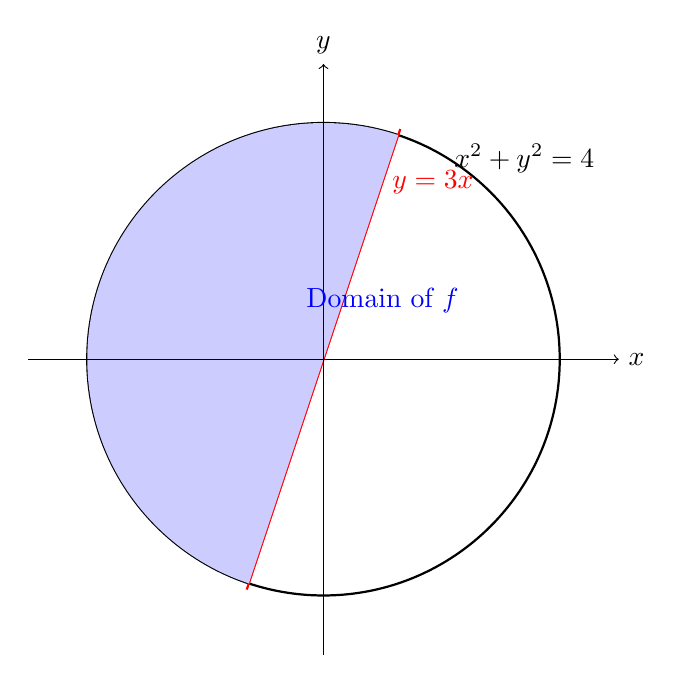
\begin{tikzpicture}[scale=1.5]
			% Draw the circle x^2 + y^2 = 4
			\draw[thick] (0,0) circle(2);
			
			% Label the circle
			\node at (1.7,1.7) {$x^2 + y^2 = 4$};
			
			% Draw the line y = 3x
			\draw[thick,red,domain=-0.65:0.65] plot (\x, {3*\x});
			
			% Label the line
			\node[red, right] at (0.5, 1.5) {$y = 3x$};
			
			% Shade the domain region
			\begin{scope}
				\clip (0,0) circle(2);
				\fill[blue!20] (-2, -6) -- (2, 6) -- (2, 2) -- (-2, 2) -- cycle;
			\end{scope}
			
			% Axes
			\draw[->] (-2.5, 0) -- (2.5, 0) node[right] {$x$};
			\draw[->] (0, -2.5) -- (0, 2.5) node[above] {$y$};
			
			% Label the domain
			\node[blue] at (0.5, 0.5) {Domain of $f$};
			
		\end{tikzpicture}
	\end{center}

	b) 
	\[ \text{Positive:} \quad  y > 3x \quad \text{and} \quad x^2 + y^{2} < 4 \] 
	\[ \text{Negative:} \quad y > 3x \quad \text{and} \quad 0 < 4 - x^{2} - y^{2} < 1 \] 
	
	
}

\newpage 
\qs{}{
	Here are several surfaces. \\
	\insertpng[0.5]{prob10a.png}
	\insertpng[0.5]{prob10b.png}
	Match each function with its graph. Justify your answers.
	\begin{enumerate}
		\item[(a)] $f(x, y) = x^2$
		\item[(b)] $f(x, y) = \sqrt{x^2 + y^2}$
		\item[(c)] $f(x, y) = e^{x^2 + y^2} - 1$
		\item[(d)] $f(x, y) = y \sin x$
		\item[(e)] $f(x, y) = \sin(x + y)$
		\item[(f)] $f(x, y) = \sin\left(\sqrt{x^2 + y^2}\right)$
	\end{enumerate}
}

\sol{
	\\
	Equation a goes with Surface V bceause it should be parabolic along the x-axis and independent of y.  \\
	Equation b goes with surface IV because the value of z should increase linearly with radical distance which should make a cone like shape \\ 
	Equation c goes with surface II z increases exponentially as x and y increase which should make for something cone like but 
	that grows faster which should make a steep smooth rise\\
	Equation d goes with surface III because the function should oscilate in the x-direction while increasing due to y values so \\
	Equation e goes with surface I because it depends on the sum of x and y and would have a constant 
	phase along lines x  + y equals a constant. So there should be a diagonal wave pattern.\\
	Equation f goes with surface VI because it should still have waves that depend on distance from origin, meaning there should be ripples. 

}
\qs{}{
	Draw a contour map of the function $f(x, y) = x^2 e^{-y}$ showing several level curves.
}

\sol{
	\[ f(x,y) = x^{2}e^{-y} \] 
	\[ x^{2}e^{-y} = k \]
	\[ e^{-y} = \frac{k}{x^{2}} \]
	\[ \ln\left( e^{-y}\right) = \ln \left( \frac{k}{x^{2}} \right)\]   
	\[ -y = \ln(k) - \ln(x^{2}) \Rightarrow y = - \ln(k) + 2\ln(x) \]
	$x^{2} > 0$ for all x in the orignal function defintion so the equation is actually 
	\[ -y = \ln(k) - \ln(x^{2}) \Rightarrow y = - \ln(k) + 2\ln(|x|) \]
	\begin{center}
		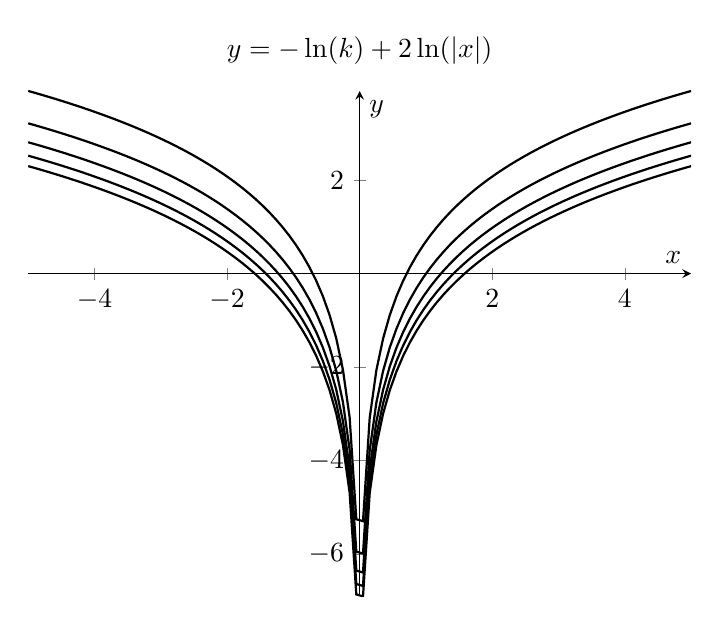
\begin{tikzpicture}
			\begin{axis}[
				axis lines = center,
				xlabel = {$x$},
				ylabel = {$y$},
				domain=-5:5,
				samples=100,
				width=10cm,
				height=8cm,
				title={$y = -\ln(k) + 2\ln(|x|)$}
			]
			% Draw several contour curves for different values of k
			\addplot [no marks, samples y=0, thick] { -ln(0.5) + 2*ln(abs(x)) }; 
			\addplot [no marks, samples y=0, thick] { -ln(1) + 2*ln(abs(x)) }; 
			\addplot [no marks, samples y=0, thick] { -ln(1.5) + 2*ln(abs(x)) }; 
			\addplot [no marks, samples y=0, thick] { -ln(2) + 2*ln(abs(x)) }; 
			\addplot [no marks, samples y=0, thick] { -ln(2.5) + 2*ln(abs(x)) }; 
			\end{axis}
		\end{tikzpicture}
	\end{center}
}

\newpage 

\qs{}{
	Match the function with its graph (labeled A-F below) and with its contour map (labeled I-VI). Give reasons for your choices.
	\begin{enumerate}
		\item[(a)] $z = e^x \cos y$
		\item[(b)] $z = \sin x - \sin y$
		\item[(c)] $z = \frac{x - y}{1 + x^2 + y^2}$
	\end{enumerate}
	\insertpng[0.6]{q12.png}
}

\newpage

\sol{\\
	a) \\
	$e^{x}$ is an exponential function in the $x$-direction, meaning that as $x$ increases the value of $z$ grow rapidly. \\
	$\cos(y)$ means that there are oscillations in the y-direction causing wave-like behavior along the $y$-axis. \\
	Graph A shows an exponential rise in the $x$-direction with some oscillations in the $y$-direction. Countour IV because of the oscillations and 
	because it is what graph A would look like from the top.  
	\\ 
	\\
	b) $\sin x - \sin y$ would have oscillations along the $x$-direction and $y$-direction. These oscillations would be of the same size as there are fixed values that 
	this equation can result in. \\
	The graph is E for this reason. Contour is III because it is a top view of the graph E and the circles are the same size which is a trait you would 
	expect.
	\\
	\\
	c)\\
	numerator of $x-y$ suggests a linear slope or difference between $x$ and $y$, so one side will be positive and the other negative. \\
	The denominator makes the effect of the numerator decrease as x and y increase since it outgrows them. So the graph of this function will have a positive peak and a negative peak near the origin 
	and then it should level out on the sides.\\
	This is why the graph is D. It is contour v because of the increasing size of the ring-like shapes as you move away from the origin which is a trait of graph d. 
}

\end{document}
